\documentclass[11pt,a4paper]{article}

% Packages
\usepackage[utf8]{inputenc}
\usepackage[spanish, es-tabla]{babel}
\usepackage{caption}
\usepackage{listings}
\usepackage{adjustbox}
\usepackage{enumitem}
\usepackage{boldline}
\usepackage{amssymb, amsmath}
\usepackage{amsthm}
\usepackage[margin=1in]{geometry}
\usepackage{xcolor}
\usepackage{soul}
\usepackage{upgreek}
\usepackage{multirow}
\usepackage{graphicx}
\usepackage{float}

% Meta
\title{Reto 1}
\author{José Antonio Álvarez}
\date{\today}

% Custom
\providecommand{\abs}[1]{\lvert#1\rvert}
\setlength\parindent{0pt}
% Redefinir letra griega épsilon.
\let\epsilon\upvarepsilon
% Fracciones grandes
\newcommand\ddfrac[2]{\frac{\displaystyle #1}{\displaystyle #2}}
% Primera derivada parcial: \pder[f]{x}
\newcommand{\pder}[2][]{\frac{\partial#1}{\partial#2}}

\lstset{    %listings config
  language=C++,
  belowcaptionskip=1\baselineskip,
  breaklines=true,
  frame=L,
  xleftmargin=0.1in,
  %otherkeywords={},
  showstringspaces=false,
  backgroundcolor=\color{white},
  basicstyle=\footnotesize\ttfamily,
  keywordstyle=\bfseries\color{purple!90!black},
  commentstyle=\itshape\color{gray!85!},
  identifierstyle=\color{blue!80!black},
  stringstyle=\color{green!60!black},
}

\begin{document}

\maketitle
\begin{enumerate}
\item \large{\textbf{Usando la notacion O, determinar la eficiencia de los siguientes segmentos de codigo:}} \\

\begin{lstlisting}
int n,j; int i=1; int x=0;           |      int n,j; int i=2; int x=0;
do{                                  |      do{
	j=1;                         |      	j=1;
	while (j <= n){              |      	while (j <= i){
		j=j*2;               |      		j=j*2;
		x++;                 |      		x++;
	}                            |      	}
	i++;                         |      	i++;
}while (i<=n); 			     | 	    }while (i<=n);
\end{lstlisting}

\begin{enumerate}

\item En el primer algoritmo podemos observar que el bucle exterior es de orden $O(n)$ mientra que el interior de orden $O(log(n))$ ya que esta realizando tantas iteraciones como potencias de 2 menores que $n$. Esto es, $log_2(n)$. Por tanto la eficiencia del algortimo completo será de orden $O(n*log(n))$

\item La única diferencia de este algoritmo (que representaremos por  $f(n)$) respecto del anterior es el tope del bucle interior. Como siempre se cumple $i \leq n$, sabemos que $O(f(n)) \leq O(n*log(n))$. También sabemos que el bucle interior depende de n. Esto es, su orden de eficiencia es estrictamente mayor que $O(1)$. Por tanto $O(n) < O(f(n))$ (recordemos que el bucle exterior ya es de orden $O(n)$. Por tanto hemos obtenido que: 
$$O(n) < O(f(n)) \leq O(n*log(n))$$ 
Como no hay ningún orden de efiencia entre $O(n)$ y $O(n*log(n))$, hemos deducido que $O(f(n)) = O(n*log(n))$.

\end{enumerate}

\item \large{\textbf{Para cada funcion $\textbf{f(n)}$ y cada tiempo $\textbf{t}$ de la tabla siguiente, determinar el mayor tamano de un problema que puede ser resuelto en un tiempo $\textbf{t}$ (suponiendo que el algoritmo para resolver el problema tarda $\textbf{f(n)}$ microsegundos, es decir, $f(n)*10^{-6}$ sg.)}} \\

\newpage

\begin{table}[!htbp]
\centering
\label{Tabla}
\begin{tabular}{|c|c|c|c|c|c|}
\hline
 \multirow{2}{*}{$f(n)$}& \multicolumn{5}{l|}{\hfil$t$} \\ \cline{2-6} 
 &  1 segundo  & 1 hora   & 1 semana   &  1 año  & 1000 años  \\ \hline
 $log_2n$ &  $\approx 10^{300000}$  &    &    &    &   \\ \hline
 $n$&   &    &    &  $\approx 3.15 \cdot 10^{15}$  &  \\ \hline
 $nlog_2n$&    &  $1.33 \cdot 10^8$  & &    &   \\ \hline
 $n^3$&    &    &   &  $146645$  &   \\ \hline
 $2^n$&  $19$  &  &    &  & \\ \hline
 $n!$&    &  $12$  &   &    &  \\ \hline
\end{tabular}
\end{table}

La primera aproximación que tuve en cuenta era meramente algorítmica, pero en seguida me di cuenta de que no podía tomar este acercamiento para $f(n) \in \{log_2(n), n\}$. Por ello realicé los siguientes cálculos: el $n$ que buscamos será el máximo de los $i$'s que cumplen: 
$$\frac{f(i)}{10^6} \leq t \leftrightarrow f(i) \leq t \cdot 10^6 \leftrightarrow i \leq f^{-1}(t \cdot 10^6)$$
Para $f(n) = log_2(n) \rightarrow f^{-1}(n) = 2^n$. Por tanto $i \leq 2^{t \cdot 10^6}$. Buscamos ahora expresarlo de la forma $10^x$:

$$10^x = 2^{t \cdot 10^6} \leftrightarrow log_{10}(10^x) = log_{10}(2^{t \cdot 10^6}) \leftrightarrow x = t \cdot 10^6 \cdot log_{10} (2). $$ 
Obteniendo: $$i \leq 10^{t \cdot 10^6 \cdot log_{10} (2). }$$
Para valores tan grandes podemos tomar la igualdad. Estudiémos ahora el segundo caso: $f(n) = n)$.

$$\frac{f(i)}{10^6} = \frac{i}{10^6} \leq t \leftrightarrow i \leq t * 10^6$$

De nuevo tomaremos la igualdad. Para el resto de casos el estudio algorítmico es viable. Aplicando un ligero cambio en el incremento de $j$ en el caso $f(n) = n \cdot log_2(n)$ para hacerlo aún más rápido conseguimos que su ejecución sea de apenas unos segundos. \\

Nota: El programa utilizado para los cálculos es el archivo adjunto \textbf{reto1.cpp}. Este es un ejemplo de ejecución:

\begin{figure}[H]
	\centering
	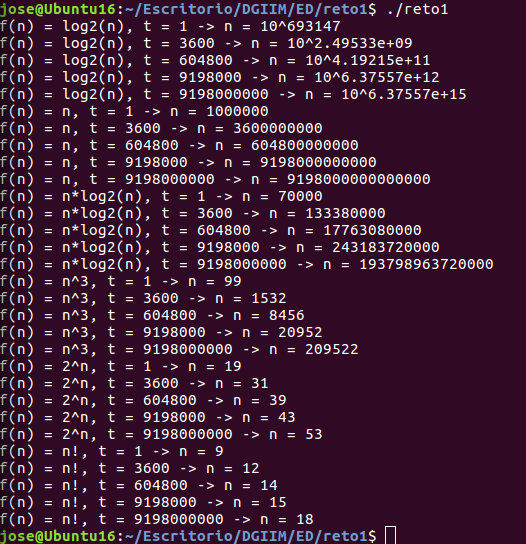
\includegraphics[width=0.8\textwidth]{Ejecucion.png}
	\caption{Cálculo final de valores de n}
\end{figure}

Por tanto la tabla queda de la siguiente forma:

\begin{table}[!htbp]
\centering
\label{Tabla}
\begin{tabular}{|c|c|c|c|c|c|}
\hline
 \multirow{2}{*}{$f(n)$}& \multicolumn{5}{l|}{\hfil$t$} \\ \cline{2-6} 
 &  1 segundo  & 1 hora   & 1 semana   &  1 año  & 1000 años  \\ \hline
 $log_2n$ &  $10^{693147}$  &  $10^{2.5 \cdot 10^9}$  &  $10^{4.19 \cdot 10^{11}}$  &  $10^{6.38 \cdot 10^{12}}$  &  $10^{6.38 \cdot 10^{15}}$ \\ \hline
 $n$&  $10^6$  &  $3.6 \cdot 10^9 $  &  $6.048 \cdot 10^{11}$  &  $9.198 \cdot 10^{12}$  & $9.198 \cdot 10^{15}$  \\ \hline
 $nlog_2n$&  $7 \cdot 10^4$  &  $1.3338 \cdot 10^8$  &  $1.776308\cdot 10^{10}$  &  $2.4318372 \cdot 10^{11}$  &  $1. 9379896372\cdot 10^{14}$ \\ \hline
 $n^3$&  $99$  &  $1532$  &  $8456$  &  $20952$  & $209522$  \\ \hline
 $2^n$&  $19$  &  $31$  & $39$   &  $43$  & $53$  \\ \hline
 $n!$&  $9$  &  $12$  &  $14$  &  $15$  &  $18$ \\ \hline
\end{tabular}
\end{table}

\end{enumerate}

\end{document}